There are many ways to understand the universe's evolution, including mapping planet orbits, dissecting the characteristics and life cycles of stars, inspecting the motion of galaxies, and analyzing interstellar dust.

\begin{eqnarray}
    & & \frac{\dot{a}^{2}(t)}{a^{2}(t)} + \frac{k c^{2}}{a^{2}(t)} - \frac{\Lambda c^{2}}{3} = \frac{8 \pi G}{3} \rho(t) \\
    & & 2 \frac{\ddot{a}(t)}{a(t)} + \frac{\dot{a}^{2}(t)}{a^{2}(t)} + \frac{k c^{2}}{a^{2}(t)} - \lambda c^{2} = - \frac{8 \pi G}{c^{2}} p(t) \, ,
\end{eqnarray}



is measured with high precision and describes many cosmological signatures, such as structure formation, the cosmic abundances of various elements such as Hydrogen and Helium, 

\begin{figure}
\centering
\begin{subfigure}{.44\textwidth}
  	\centering
  	\includegraphics[trim={22.0cm, 1.0cm, 15cm, 1.5cm}, clip, width=\linewidth]{Figures/polModCartoon.jpg}
   	\caption{\label{fig:polModCartoon}}
\end{subfigure}%
\begin{subfigure}{.56\textwidth}
  	\centering
  	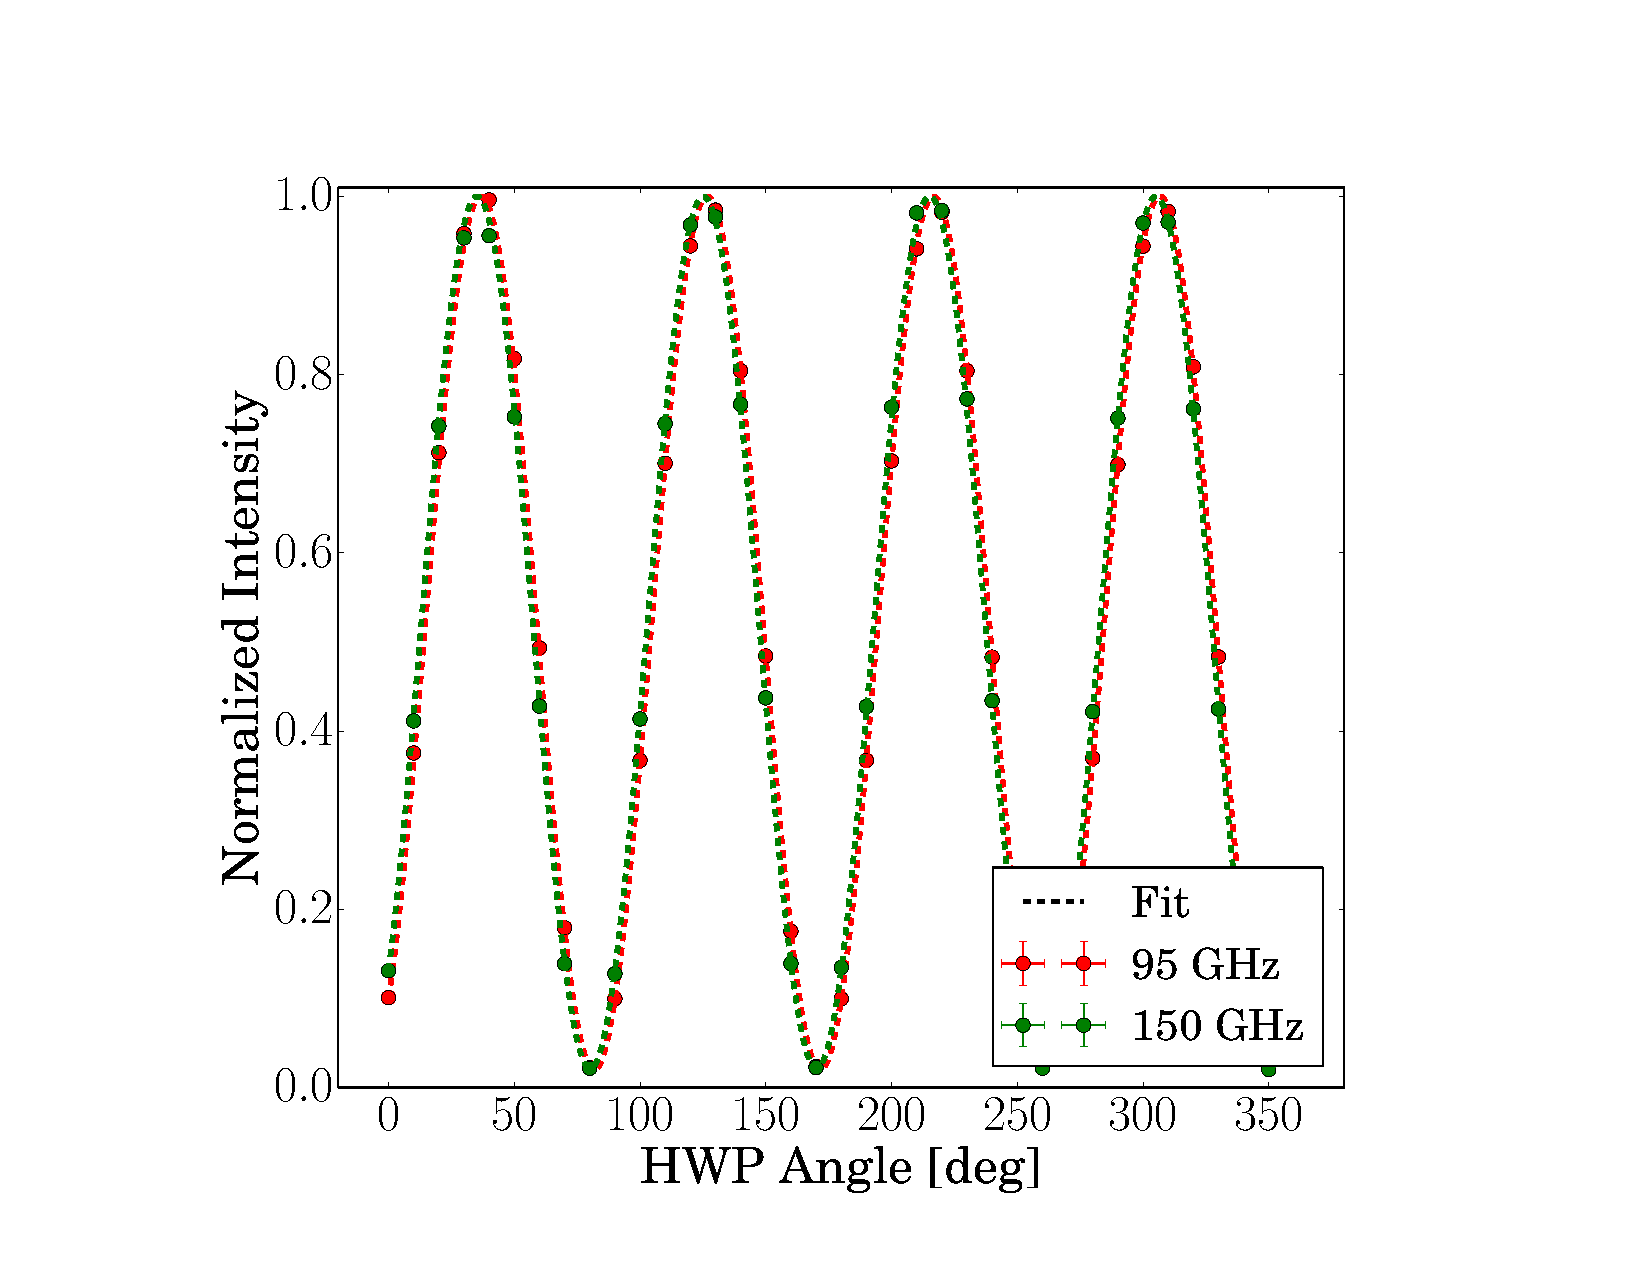
\includegraphics[trim={3.0cm, 1.0cm, 3.5cm, 1.5cm}, clip, width=\linewidth]{Figures/polMod.pdf}
  	\caption{\label{fig:polModPlot}}
\end{subfigure}
\caption{Measurement of the PB2 HWP polarization performance in the PB2 frequency bands. \ref{fig:polModCartoon} shows a cartoon of the polarized measurement apparatus. The HWP is mounted on a rotating stage to modulate a polarized thermal source with respect to a polarized detector. \ref{fig:polModPlot} shows normalized intensity as a function of HWP angle in each PB2 frequency band. The points are the data and the dotted lines are the fits to Equation \ref{eq:fitPol}. The 95 GHz modulation (in red) is slightly ahead of the 150 GHz modulation (in green). The error bars for the measured data points are small and hence are hidden in this plot. \label{fig:polMod}}
\end{figure}

\begin{figure}
\centering
\begin{subfigure}{.49\textwidth}
  	\centering
  	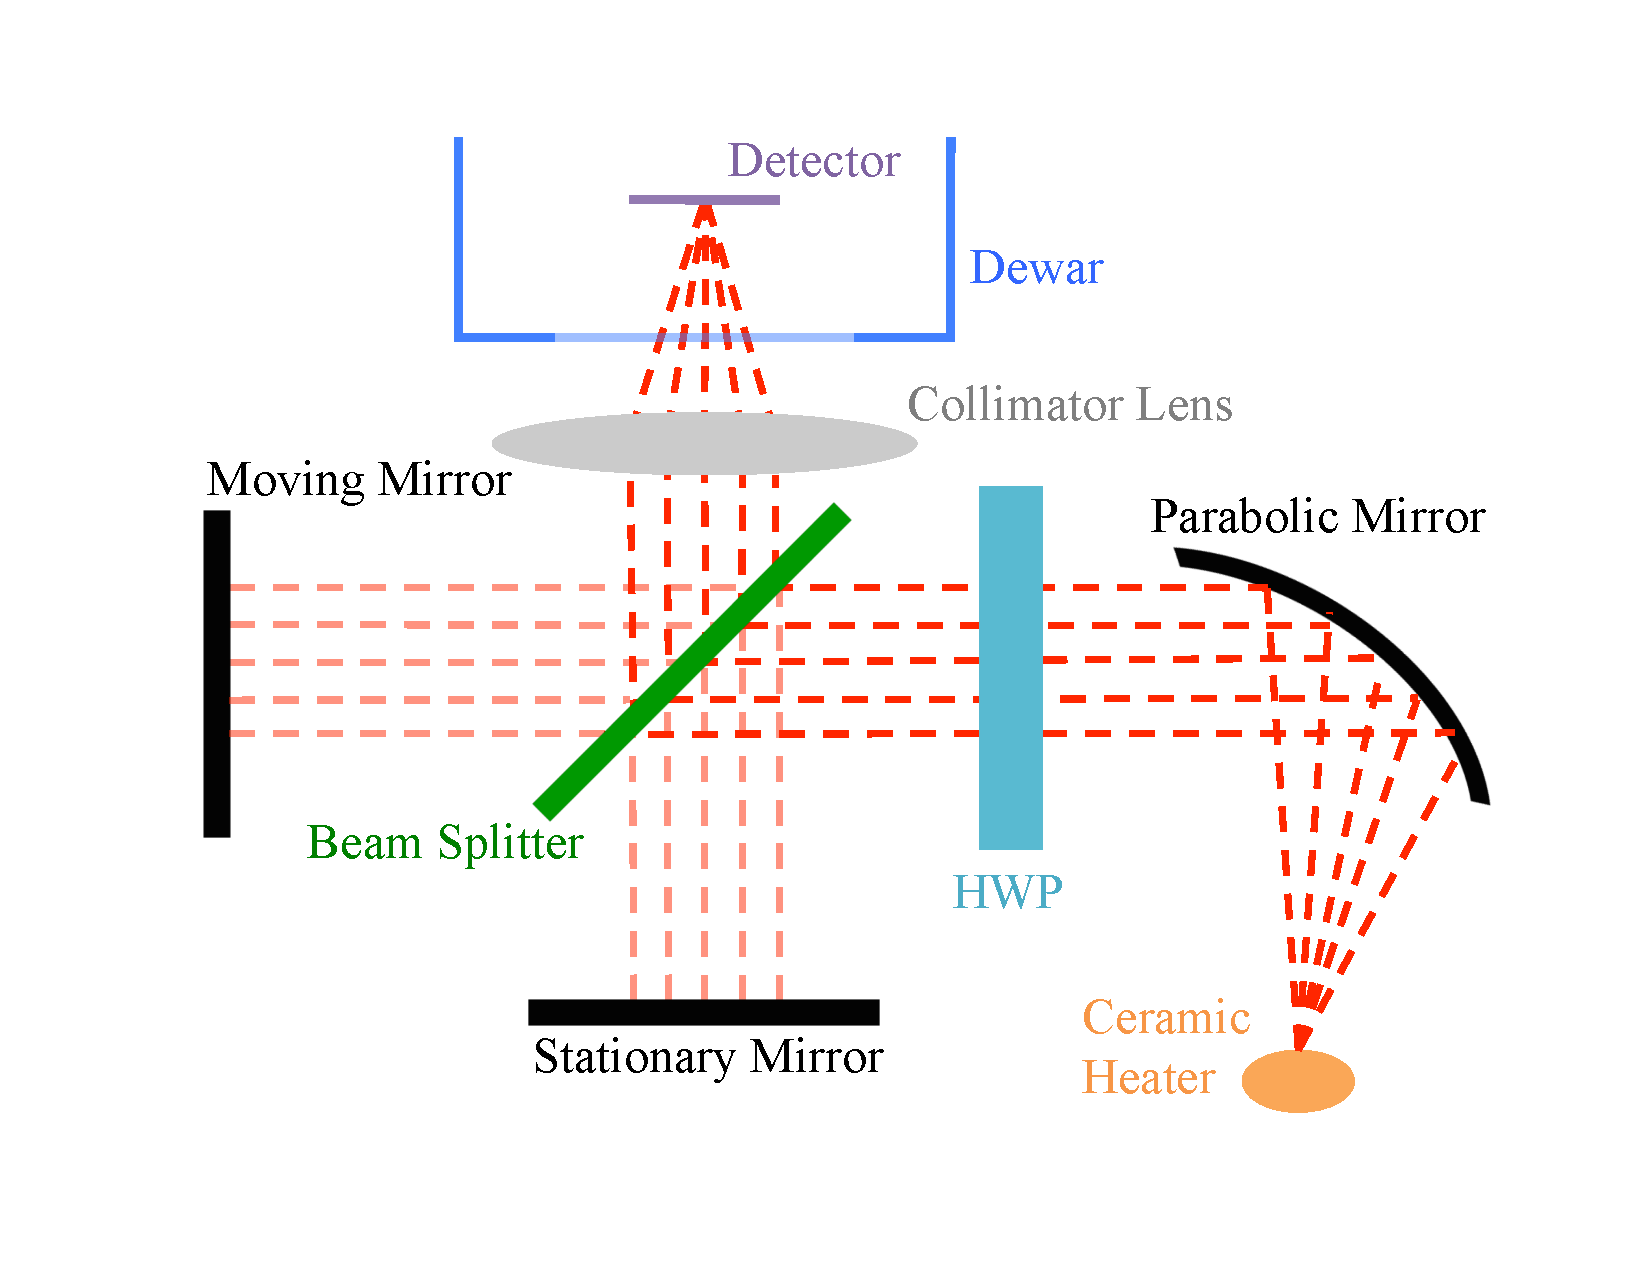
\includegraphics[trim={1.5cm, -2.0cm, 1.5cm, 1.5cm}, clip, width=\linewidth]{Figures/FTSCartoon.jpg}
   	\caption{\label{fig:FTS}}
\end{subfigure}%
\begin{subfigure}{.51\textwidth}
  	\centering
  	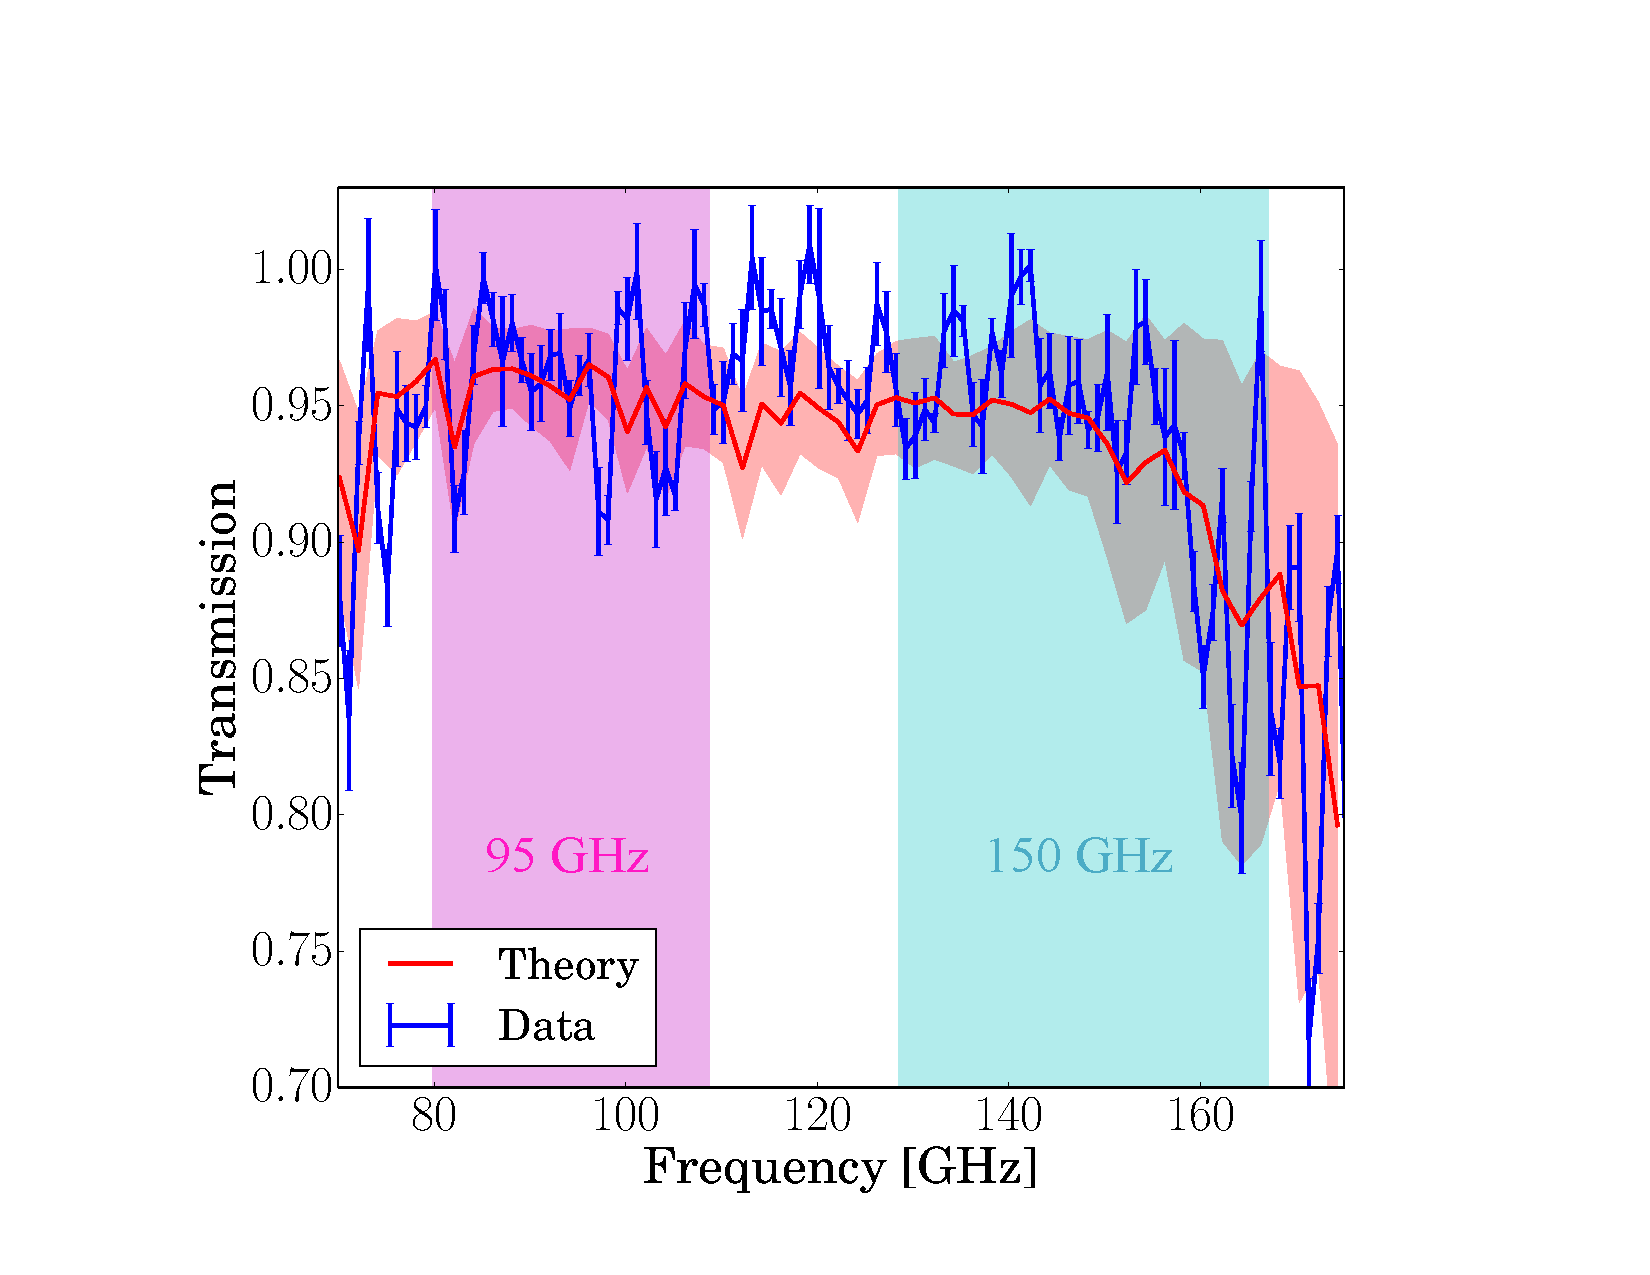
\includegraphics[trim={1.5cm, 1.3cm, 1.5cm, 1.5cm}, clip, width=\linewidth]{Figures/HWPBandpass.pdf}
  	\caption{\label{fig:hwpBandpass}}
\end{subfigure}
\caption{Measurement of the transmission through the PB2 HWP. \ref{fig:FTS} shows a cartoon of the FTS apparatus used to measure the HWP transmission. Signal from a temperature-modulated source is collimated, travels through the HWP and into the FTS, and is focused onto a cryogenic test pixel. \ref{fig:hwpBandpass} shows the result of the measurement in blue and the theoretical transmission curve constructed from the parameters listed in Table \ref{table:measOptics} in red. The measurement and the theory agree to within 1$\sigma$ uncertainty. \label{fig:bandpass}}
\end{figure}

\begin{figure}
\centering
	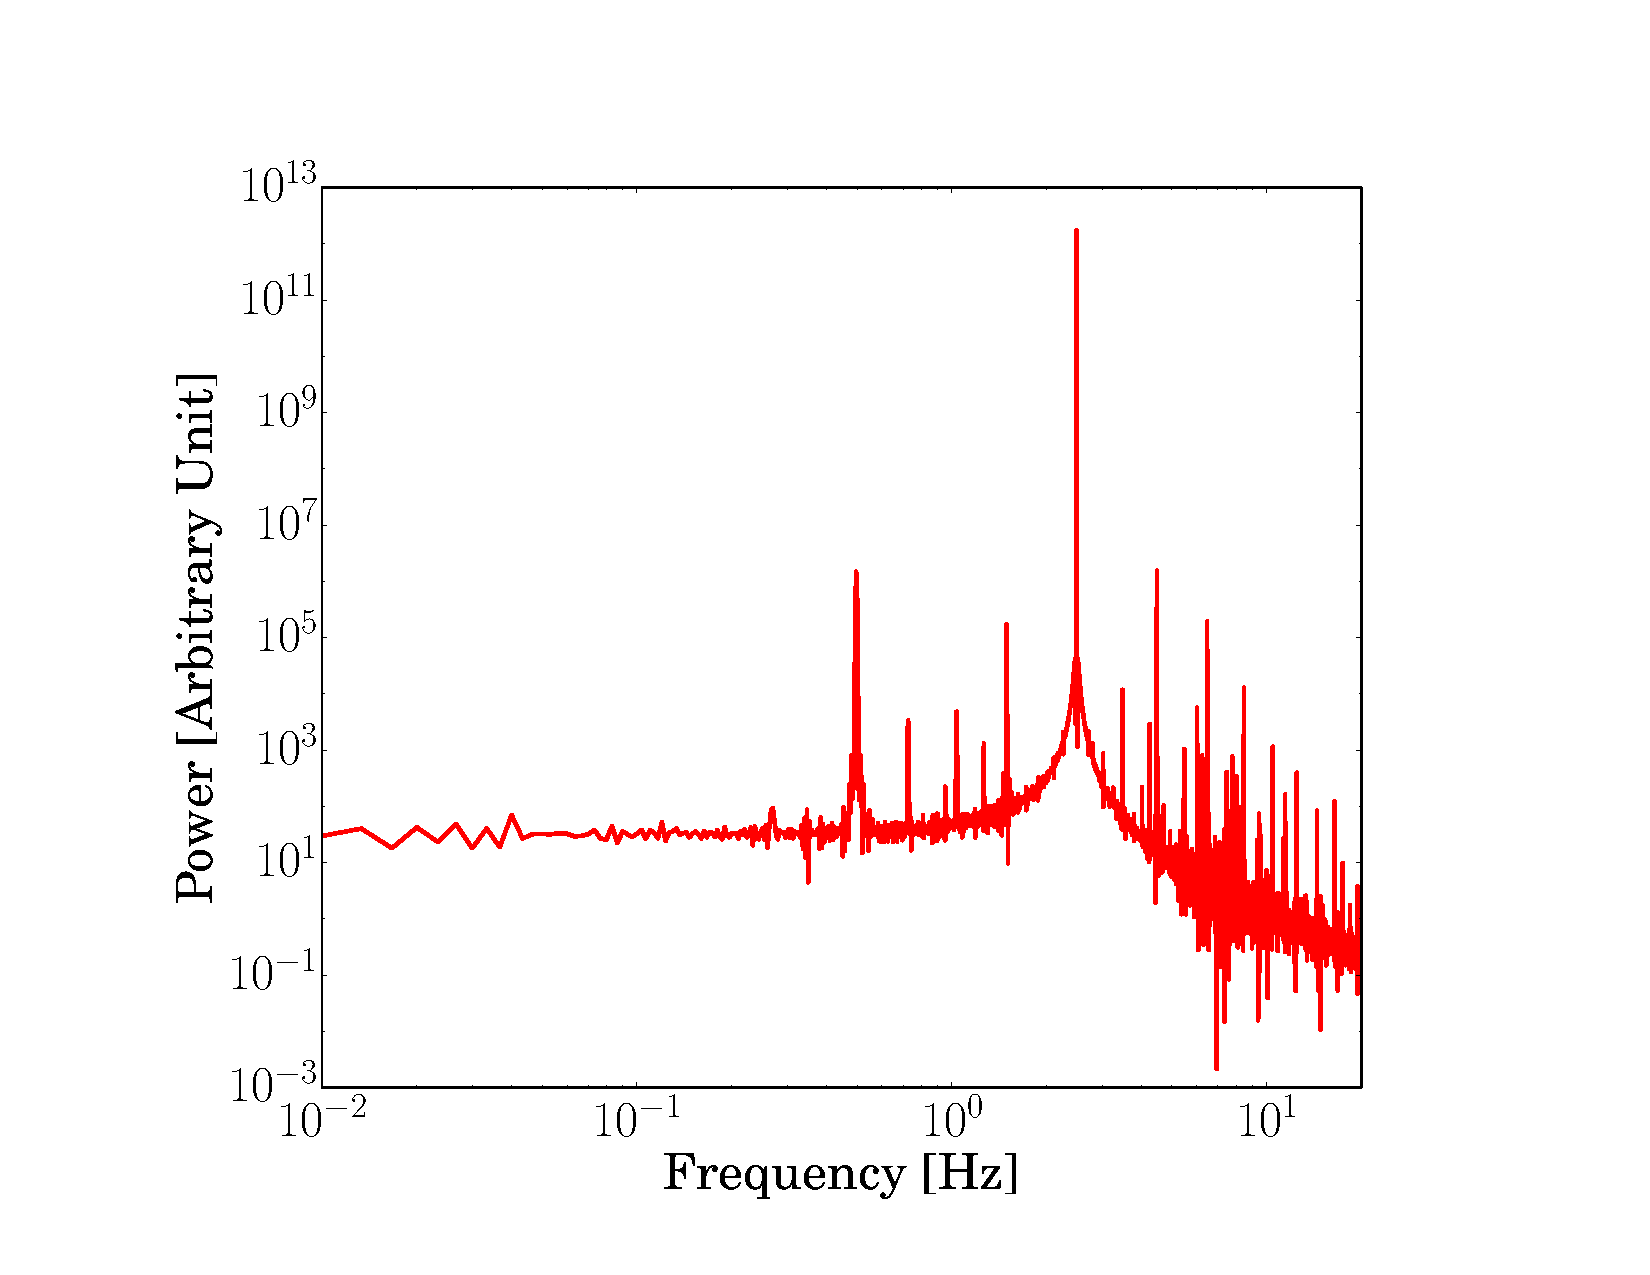
\includegraphics[trim={1.5cm, 1.0cm, 1.5cm, 1.5cm}, clip, width=0.7\linewidth]{Figures/DrivePSD.pdf}
	\caption{A power spectral density of the HWP rotation at $\approx$ 2.2 Hz over a five-minute period. The excellent rotational stability of the drive train demonstrates the effectiveness of the servo/timing belt system. \label{fig:motorPSD}}
\end{figure}

\begin{figure}[h!]
\centering
\begin{subfigure}
  	\centering
  	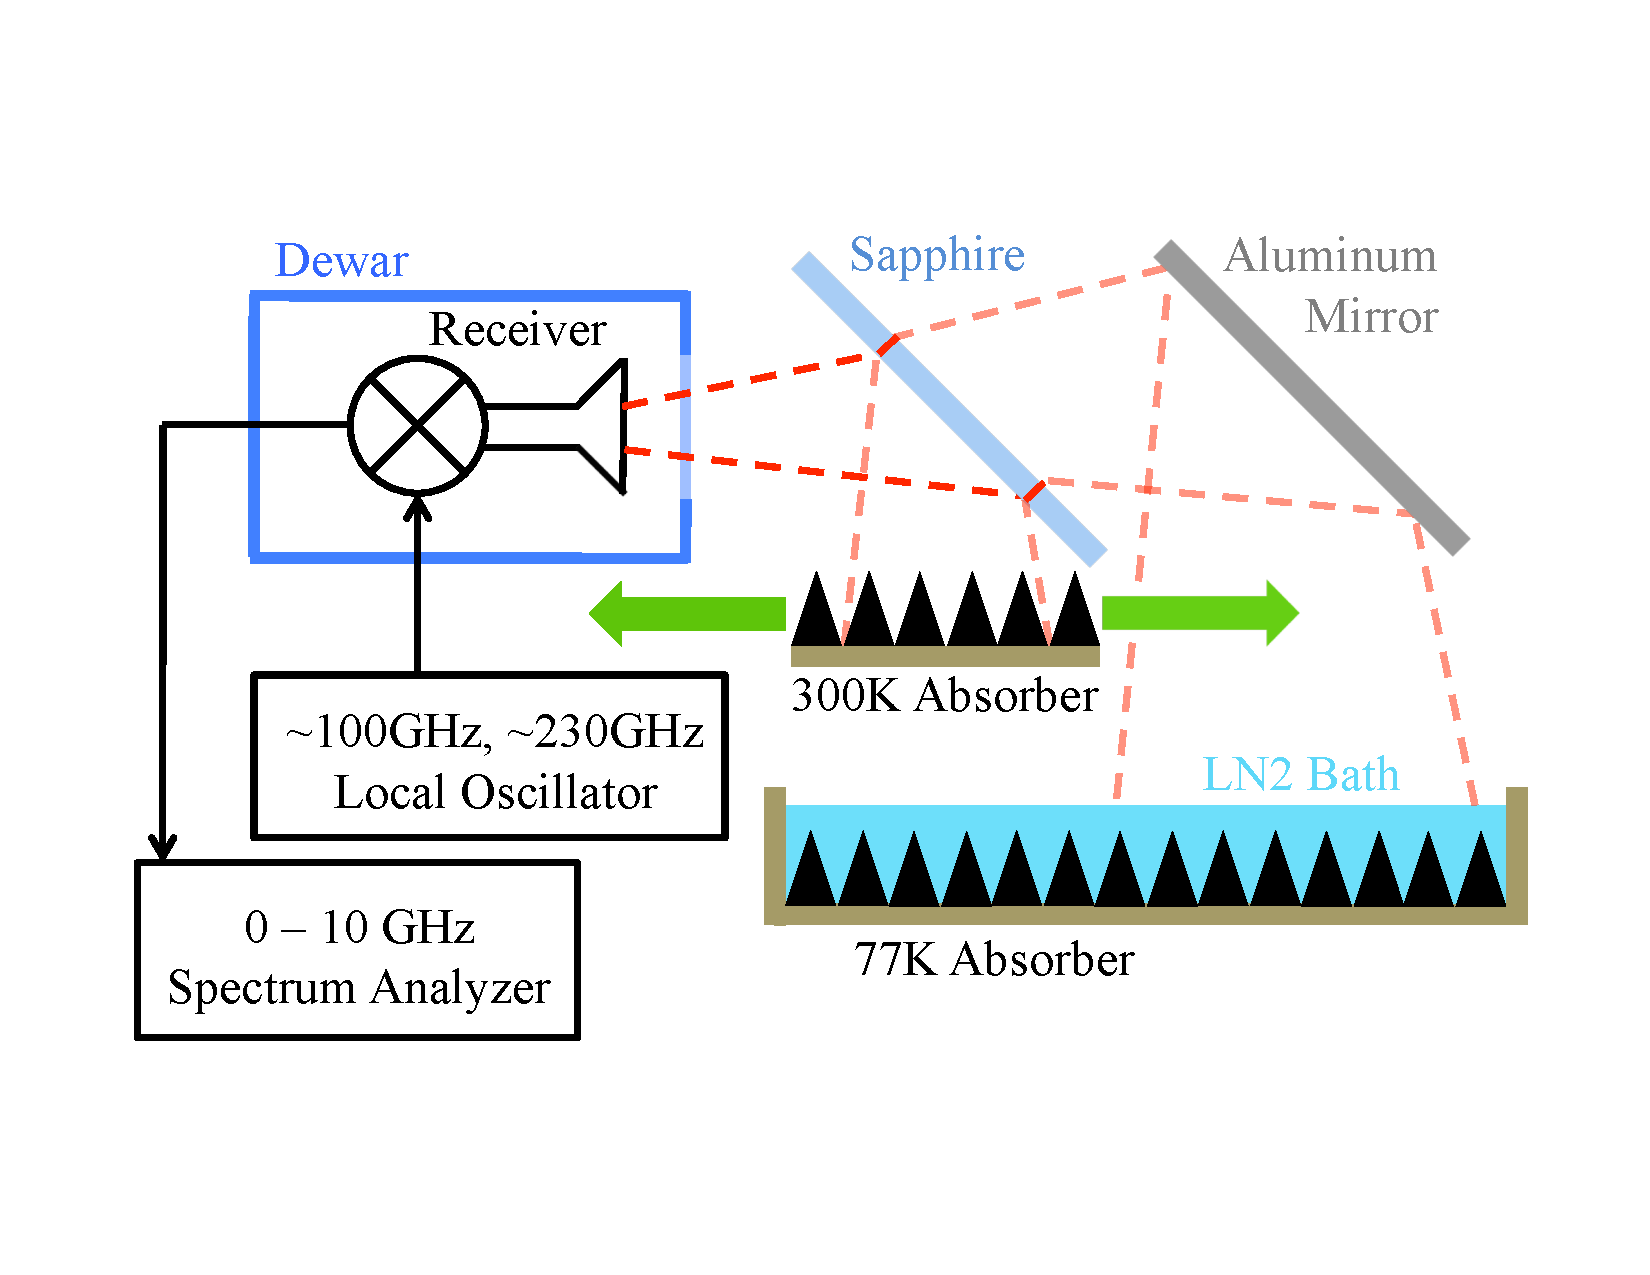
\includegraphics[trim={1.5cm, 2.5cm, 1.5cm, 2.5cm}, clip, width=\linewidth]{Figures/TEA.jpg}
   	\caption{\label{fig:tea}}
\end{subfigure}%
\begin{subfigure}
  	\centering
  	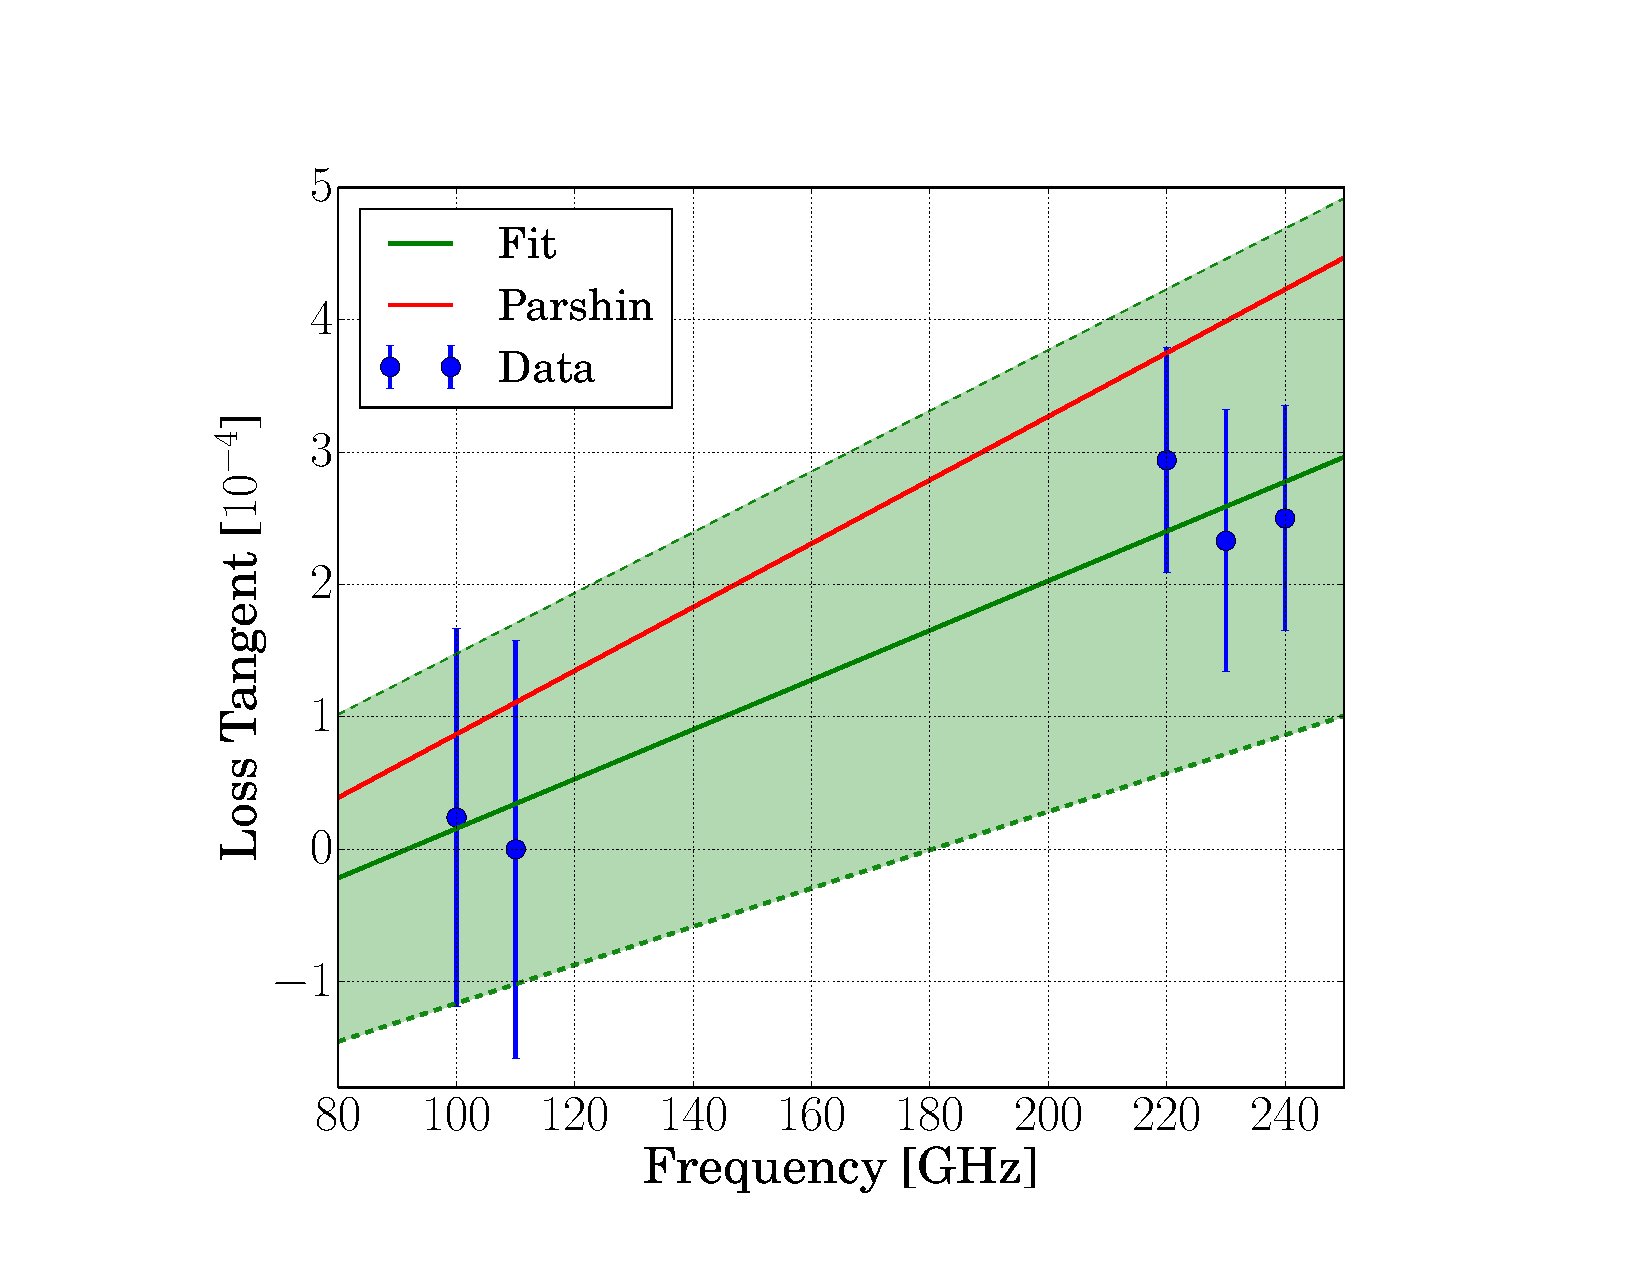
\includegraphics[trim={1.5cm, 1.0cm, 1.5cm, 2.5cm}, clip, width=\linewidth]{Figures/SapphireLoss.pdf}
  	\caption{\label{fig:sappLT}}
\end{subfigure}
\caption{PB2 HWP sapphire tan $\delta$ is measured using the TEA shown schematically in \ref{fig:tea}. Thermal emission from the sapphire slab is measured over a 77 K background using a heterodyne receiver. A series of configurations involving 300 K absorber are used to calibrate receiver gain, receiver noise, reflection from the sapphire, and transmission through the sapphire. \ref{fig:sappLT} shows a measurement of the IF-band-averaged, axes-averaged GHTOT sapphire tan $\delta$ at 5 LO frequencies with error bars that account for both statistical and systematic uncertainty in blue, a linear fit to those data points in green, and data presented in Parshin et al. \cite{parshin} in red. \label{fig:Sapphire}}
\end{figure}

\begin{figure}[!ht]
    \centering
    \subfloat[\label{fig:inflation:a}]{
        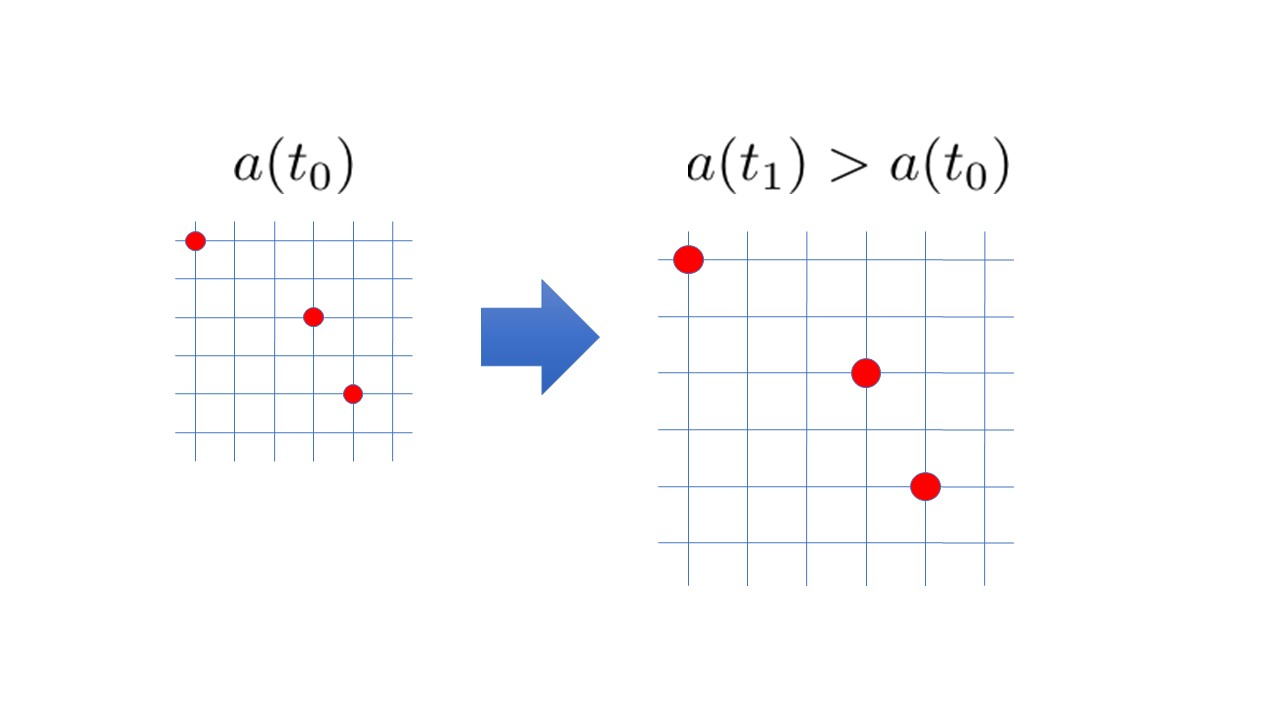
\includegraphics[width=0.45\linewidth, trim=3cm 0cm 4cm 0cm, clip]{Introduction/Figures/scale_factor.jpg}
    }
    \hfill
    \subfloat[\label{fig:inflation:b}]{
        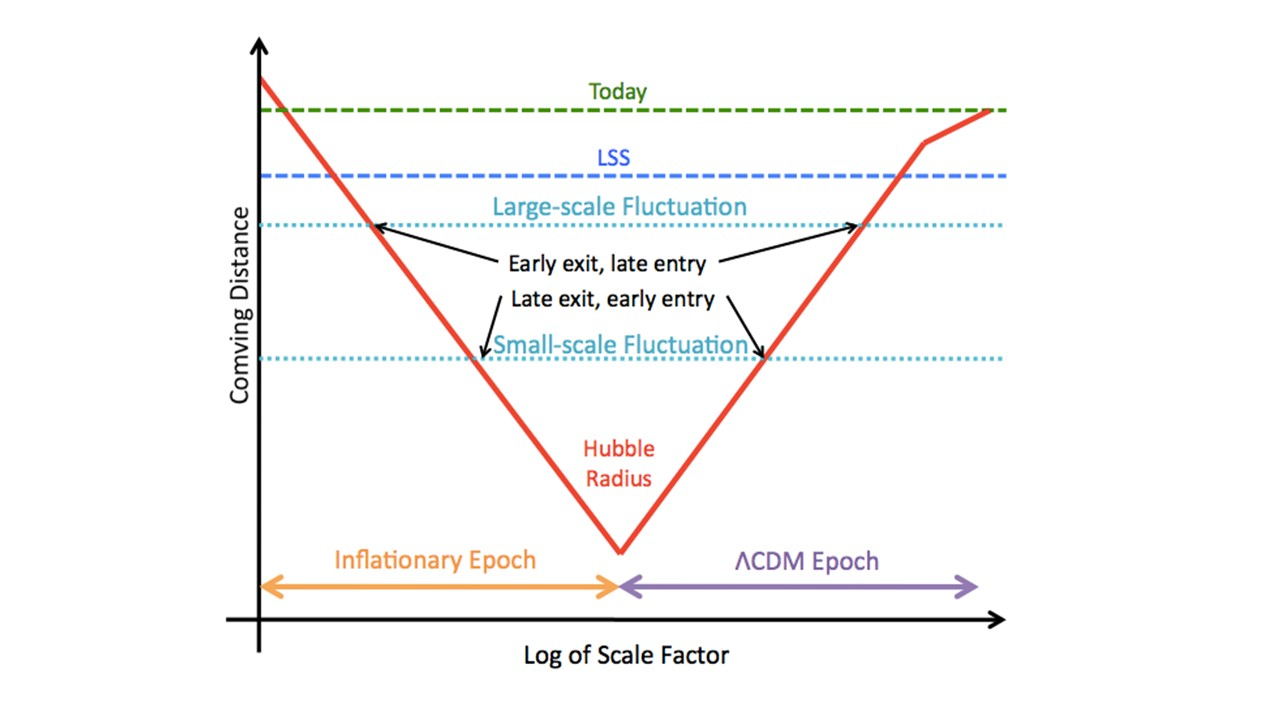
\includegraphics[width=0.45\linewidth, trim=6cm 1cm 6cm 1cm, clip]{Introduction/Figures/inflation_modes.jpg}
    }
    \caption[Cartoon depiction of the scale factor and how inflation it and comoving distance]{Cartoon explanation of the geometry of inflation. \ref{fig:inflation:a} shows a a grid, which represents space, populated by three dots, representing specific locations on the spatial grid. As the scale factor grows over time, so does the spacing of the grid, and therefore the distance and velocity between the red dots. \ref{fig:inflation:b} shows qualitatively the relationship between the Hubble Radius---or equivalently the causal horizon---in units of comoving distance vs the scale factor---or equivalently time---during both the inflationary and standard cosmological epochs. During inflation, the Hubble radius shrinks, freezing length scales that were once in causal contact outside the causal horizon. During the standard cosmological evolution, the Hubble radius grows, and these scales reenter the horizon, allowing them to evolve. The horizontal lines show that small-scale fluctuations exit/enter the horizon first while large-scale fluctuations exit/enter the horizon last. The last scattering surface (LSS) is shown by a blue dotted line, and the kink in the Hubble radius at late times represents the transition from a radiation-dominated universe to a matter-dominated one.}
    \label{fig:inflation}
\end{figure}

This model of an eternal universe gets around the problems of a multiverse and the need for a ``creation moment'' while also describing the structure and CMB fluctuations that we see today.

The larger the fluctuations, the larger the measurement variance.

%%%%%%%%%%%%%%%%%%%%%%%%%%%%%%%%
%%%%%%%%%%%%%%%%%%%%%%%%%%%%%%%%
%%%%%%%%%%%%%%%%%%%%%%%%%%%%%%%%

\section{CMB polarization}
\label{sec:cmb_polarization}

\begin{figure}[!t]
    \centering
    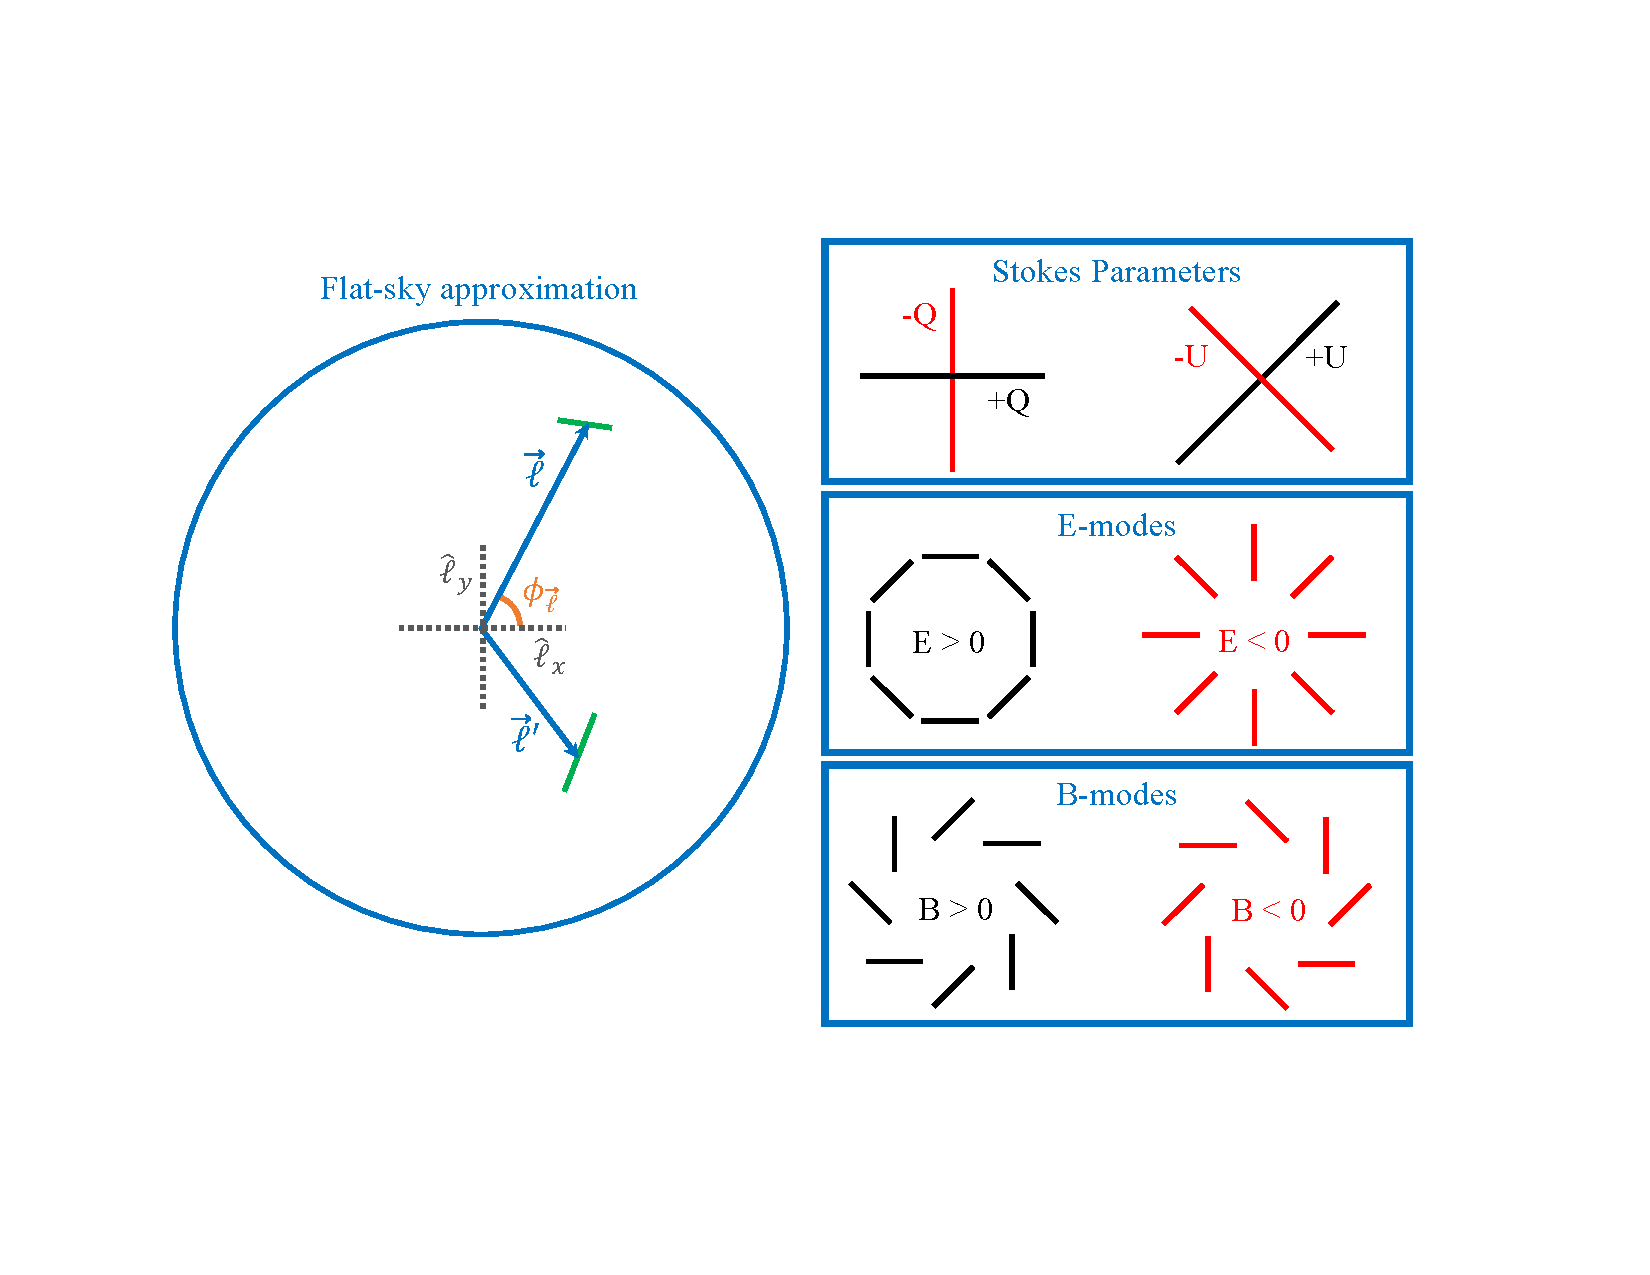
\includegraphics[width=\linewidth, trim=4cm 1cm 3cm 2cm, clip]{Introduction/Figures/emodes_bmodes.pdf}
    \caption[Stokes parameters, E-modes, B-modes in the flat-sky approximation]{A cartoon depiction of how quadrupolar anisotropies in the CMB intensity give rise to E-mode and B-mode polarization patterns. The top figures, adapted from a 1997 paper by Wayne Hu and Martin White \cite{hu_cmb_1997}, show the $m = 0$ mode of a $\ell = 2$ anisotrophy, which is called a scalar mode, and the $m = 2$ mode of a $\ell = 2$ anisotropy, which is called a tensor mode. The shaded arrows denote the wave propagation direction. The bottom figures show the zero-curl E-mode polarization pattern and the zero-divergence B-mode polarization pattern. Both scalar and tensor anisotropies give rise to E-modes, but only tensor perturbtions give rise to B-modes.}
    \label{fig:emodes_bmodes}
\end{figure}

An indeed, up until recently with the advent of precision polarimetry, the constraint on $r$ was predominantly due to temperature information. 

